\section{Theory}
\subsection{Spontaneous parametric downconversion} 
Spontaneous parametric downconversion is the spontaneous splitting of a photon in two different photons. That can be done by shining with a laser beam on a crystal, which has nonlinear effects. Under certain circumstances the both emitted photons of the crystal are entangled. 
As for every process momentum and energy conservation must be fulfilled. Because the energy for a photon is $E = \hbar \omega$, one can consider the frequencies to satisfiy the energy conservation. The pumping laser from the laser has the frequency $\omega_{\mathrm{p}}$. The resulting photons, which are named as signal and idler photon, after the splitting must have frequencies below $\omega_{\mathrm{p}}$. The energy conservation can be written as
\begin{equation}
    \omega_{\mathrm{p}} = \omega_{\mathrm{i}} + \omega_{\mathrm{s}},
\end{equation}
where $\omega_{\mathrm{i}}$ is the frequency of the idler photon and $\omega_{\mathrm{s}}$ of the signal photon. Here we are interested in the degenerated case $ \omega_{\mathrm{s}} = \omega_{\mathrm{i}}$ to make the photons indistinguishable by frequency. 
As the momentum can be calculated by $\vec{p} = \hbar \vec{k}$, for  the momentum conversation one con consider the $\vec{k}$ vectors of the tree photons. One obtains
\begin{equation}
    \vec{k}_{\mathrm{p}} =  \vec{k}_{\mathrm{i}}  + \vec{k}_{\mathrm{s}},
    \label{eq:phase_matching}
\end{equation}
what is called phase matching. 
The explained process is not possible for free electrons, but in a nonlinear medium. The nonlinearity refers to the polarization which is not linear dependent on the electric field
\begin{equation}
    \vec{P}_{\mathrm{i}} = \varepsilon_0 \left( \chi^{(1)} \vec{E}_{\mathrm{j}} 
    + \chi^{(2)} \vec{E}_1 \vec{E}_2 
    + \chi^{(3)} \vec{E}_1 \vec{E}_2 \vec{E}_3 + ... \right).
\end{equation}
The understand phase matching it is important to understand how photons propagate in a birefringence media. In this experiment a Beta Barium Borate (BBO) crystal is used which is an anisotropic medium. A BBO crystal is an uniaxiale crystal and the special symmetry axis is called optical axis (OA).  Because of that there are two different refractive indices. They are called ordinary $(n_{\mathrm{o}})$ and extraordinary $(n_{\mathrm{e}})$. 
If the polarization of the photons is parallel to the OA, the photons will see only $(n_{\mathrm{e}})$. 
For the case that the polarization is perpendicular to the OA, the photons will see only $(n_{\mathrm{o}})$. When the polarization is something bewteen this to cases, the refractice index can be calculated with
\begin{equation}
    n_{\mathrm{e}}(\lambda, \vartheta_{\mathrm{e}}) 
    = \left( 
    \frac{\mathrm{cos}^2(\vartheta_{\mathrm{e}})}{n_{\mathrm{o}}^2(\lambda)} 
    + \frac{\mathrm{sin}^2(\vartheta_{\mathrm{e}})}{n_{\mathrm{e}}^2(\lambda)}
    \right)^{-\frac{1}{2}},
\end{equation}
where $\lambda$ is a hidden parameter. What a hidden parameter is, is explained in chapter \ref{sec:theory_CHSH}.  
The $\vec{k}$ vectors are related to the refractive indices. These relations can be inserted in the euqation for the phase matching \eqref{eq:phase_matching}. The result is, that the emission directions of the two created photons habe to be fixed, to fulfill equaion \eqref{eq:phase_matching}. To get two entangled photonss, the pumping photon has to be extraordinary polarised. Then one emmited photon is extraordinary and the other one is ordinary polarised. That results in a fixed emission angle of the created entangled photon pair and the geomytry of two cones, see figure \ref{fig:theory_cones}. 
\begin{figure}[H]
\centering
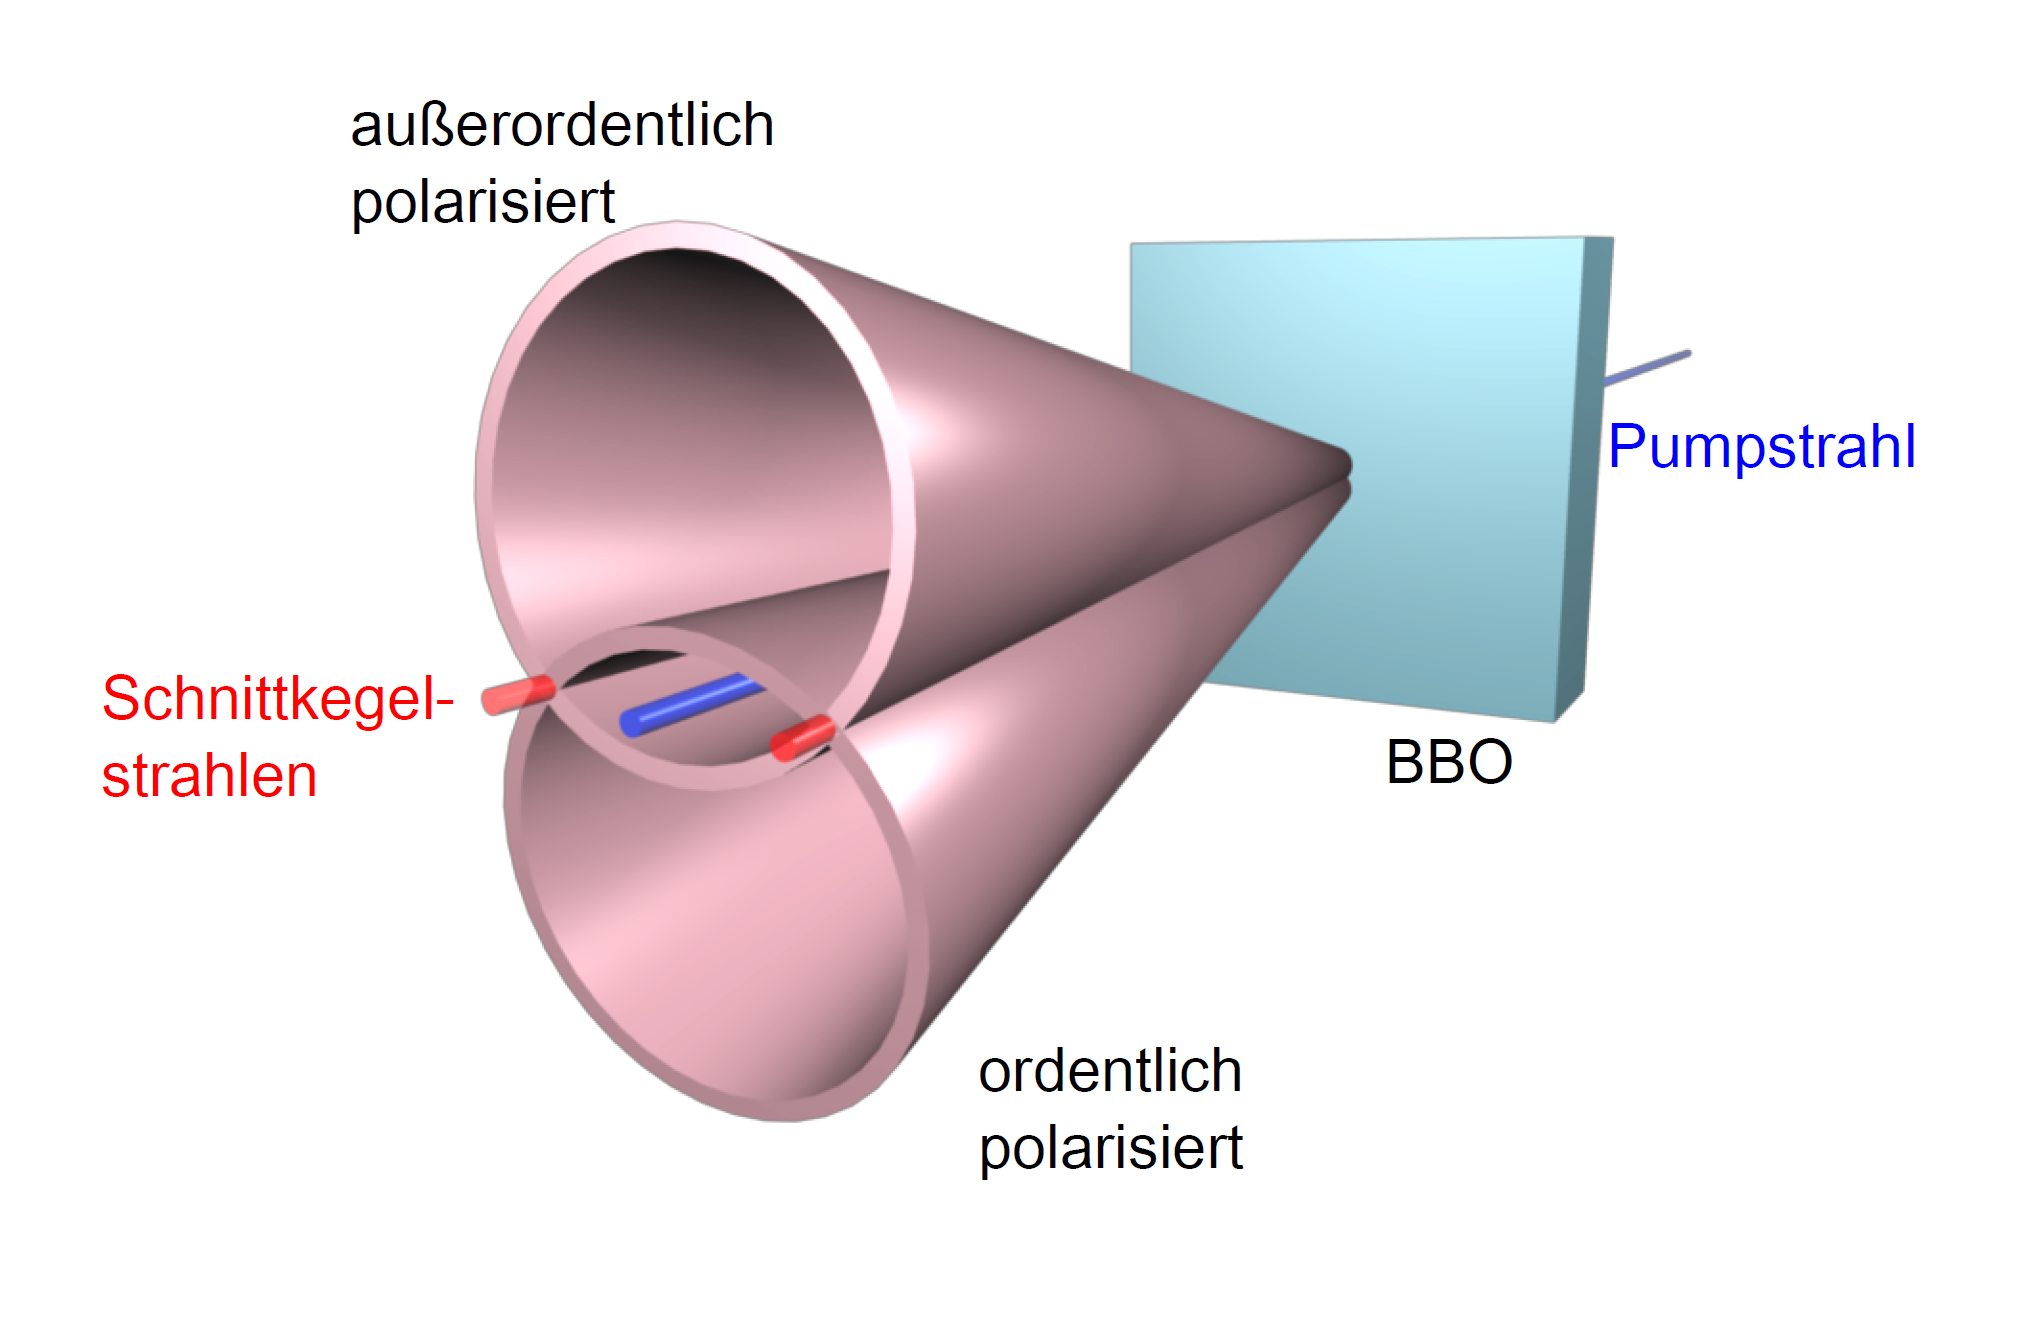
\includegraphics[scale=0.2]{figures/2_kegel.PNG}
\caption{Scetch of spontaneous parametric downconversion with the two cones for the extraordinary and ordinary polarised photon \cite{barz}.   }
\label{fig:theory_cones}
\end{figure}

%Talk:
%   - both walk off effect --> oder im Versuchsaufbau Teil
\subsection{CHSH inequality}\label{sec:theory_CHSH}
%TALK about:
%   - bell states
%   - entanglement
%   - hanbury brown twiss effect
%   - inequality
%   - how to violate inequality
%   - hidden parametr lambda
